\section{Introduction to Buildroot}

\begin{frame}{Buildroot at a glance}
  \begin{itemize}
  \item Can build a toolchain, a rootfs, a kernel, a bootloader
  \item {\bf Easy to configure}: menuconfig, xconfig, etc.
  \item {\bf Fast}: builds a simple root filesystem in a few minutes
  \item Easy to understand: written in make, extensive documentation
  \item {\bf Small} root filesystem, starting at 2 MB
  \item {\bf 2800+ packages} for user space libraries/apps available
  \item {\bf Many architectures} supported
  \item {\bf Well-known technologies}: {\em make} and {\em kconfig}
  \item Vendor neutral
  \item Active community, regular releases
    \begin{itemize}
    \item The present slides cover {\em Buildroot 2021.02}. There may
      be some differences if you use older or newer Buildroot versions.
    \end{itemize}
  \item \url{https://buildroot.org}
  \end{itemize}
\end{frame}

\begin{frame}{Buildroot design goals}
  \begin{itemize}
  \item Buildroot is designed with a few key goals:
    \begin{itemize}
    \item Simple to use
    \item Simple to customize
    \item Reproducible builds
    \item Small root filesystem
    \item Relatively fast boot
    \item Easy to understand
    \end{itemize}
  \item Some of these goals require to not necessarily support all
    possible features
  \item They are some more complicated and featureful build systems
    available (Yocto Project, OpenEmbedded)
  \end{itemize}
\end{frame}

\begin{frame}{Who's using Buildroot?}
  \begin{columns}
    \column{0.6\textwidth}
    \begin{itemize}
    \item {\bf System makers}
      \begin{itemize}
      \item SpaceX
      \item Tesla
      \item GoPro
      \item Barco
      \item Rockwell Collins
      \end{itemize}
    \item {\bf Processor vendors}
      \begin{itemize}
      \item Marvell
      \item Microchip
      \item Rockchip
      \end{itemize}
    \item {\bf SoM and board vendors}
    \item Many companies when doing {\em R\&D} on products
    \item Many, many {\bf hobbyists} on development boards:
      Raspberry Pi, BeagleBone Black, etc.
  \end{itemize}
  \column{0.4\textwidth}
  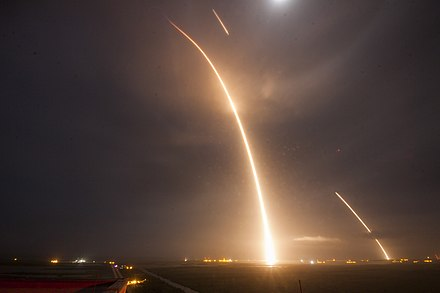
\includegraphics[width=0.5\textwidth]{slides/buildroot-introduction/spacex.jpg}\includegraphics[width=0.5\textwidth]{slides/buildroot-introduction/tesla.jpg}\\
  \includegraphics[width=0.5\textwidth]{slides/buildroot-introduction/armada.jpg}\includegraphics[width=0.5\textwidth]{slides/buildroot-introduction/raspberrypi.jpg}
  \end{columns}
\end{frame}

\begin{frame}{Getting Buildroot}
  \begin{itemize}
  \item Stable Buildroot releases are published every three months
    \begin{itemize}
    \item \code{YYYY.02}, \code{YYYY.05}, \code{YYYY.08},
      \code{YYYY.11}
    \end{itemize}
  \item Tarballs are available for each stable release
    \begin{itemize}
    \item \url{https://buildroot.org/downloads/}
    \end{itemize}
  \item However, it is generally more convenient to clone the Git
    repository
    \begin{itemize}
    \item Allows to clearly identify the changes you make to the
      Buildroot source code
    \item Simplifies the upstreaming of the Buildroot changes
    \item \code{git clone git://git.buildroot.net/buildroot}
    \item Git tags available for every stable release.
    \end{itemize}
  \item One {\bf long term support} release published every year
    \begin{itemize}
    \item Maintained during one year
    \item Security fixes, bug fixes, build fixes
    \item Current LTS is release is \code{2021.02}, maintained until
      March-April 2022, next one will be \code{2022.02}.
    \end{itemize}
  \end{itemize}
\end{frame}

\begin{frame}[fragile]{Using Buildroot}
  \begin{itemize}
  \item Implemented in \code{make}
    \begin{itemize}
    \item With a few helper shell scripts
    \end{itemize}
  \item All interaction happens by calling \code{make} in the main Buildroot
    sources directory.
    \begin{block}{}
\begin{verbatim}
$ cd buildroot/
$ make help
\end{verbatim}
    \end{block}
  \item No need to run as \code{root}, Buildroot is designed to be
    executed with normal user privileges.
    \begin{itemize}
    \item Running as root is even strongly discouraged!
    \end{itemize}
  \end{itemize}
\end{frame}

\begin{frame}{Configuring Buildroot}
  \begin{itemize}
  \item Like the Linux kernel, uses {\em Kconfig}
  \item A choice of configuration interfaces:
    \begin{itemize}
    \item \code{make menuconfig}
    \item \code{make nconfig}
    \item \code{make xconfig}
    \item \code{make gconfig}
    \end{itemize}
  \item Make sure to install the relevant libraries in your system
    ({\em ncurses} for menuconfig/nconfig, {\em Qt} for xconfig, {\em
      Gtk} for gconfig)
  \end{itemize}
\end{frame}

\begin{frame}{Main {\tt menuconfig} menu}
  \begin{center}
    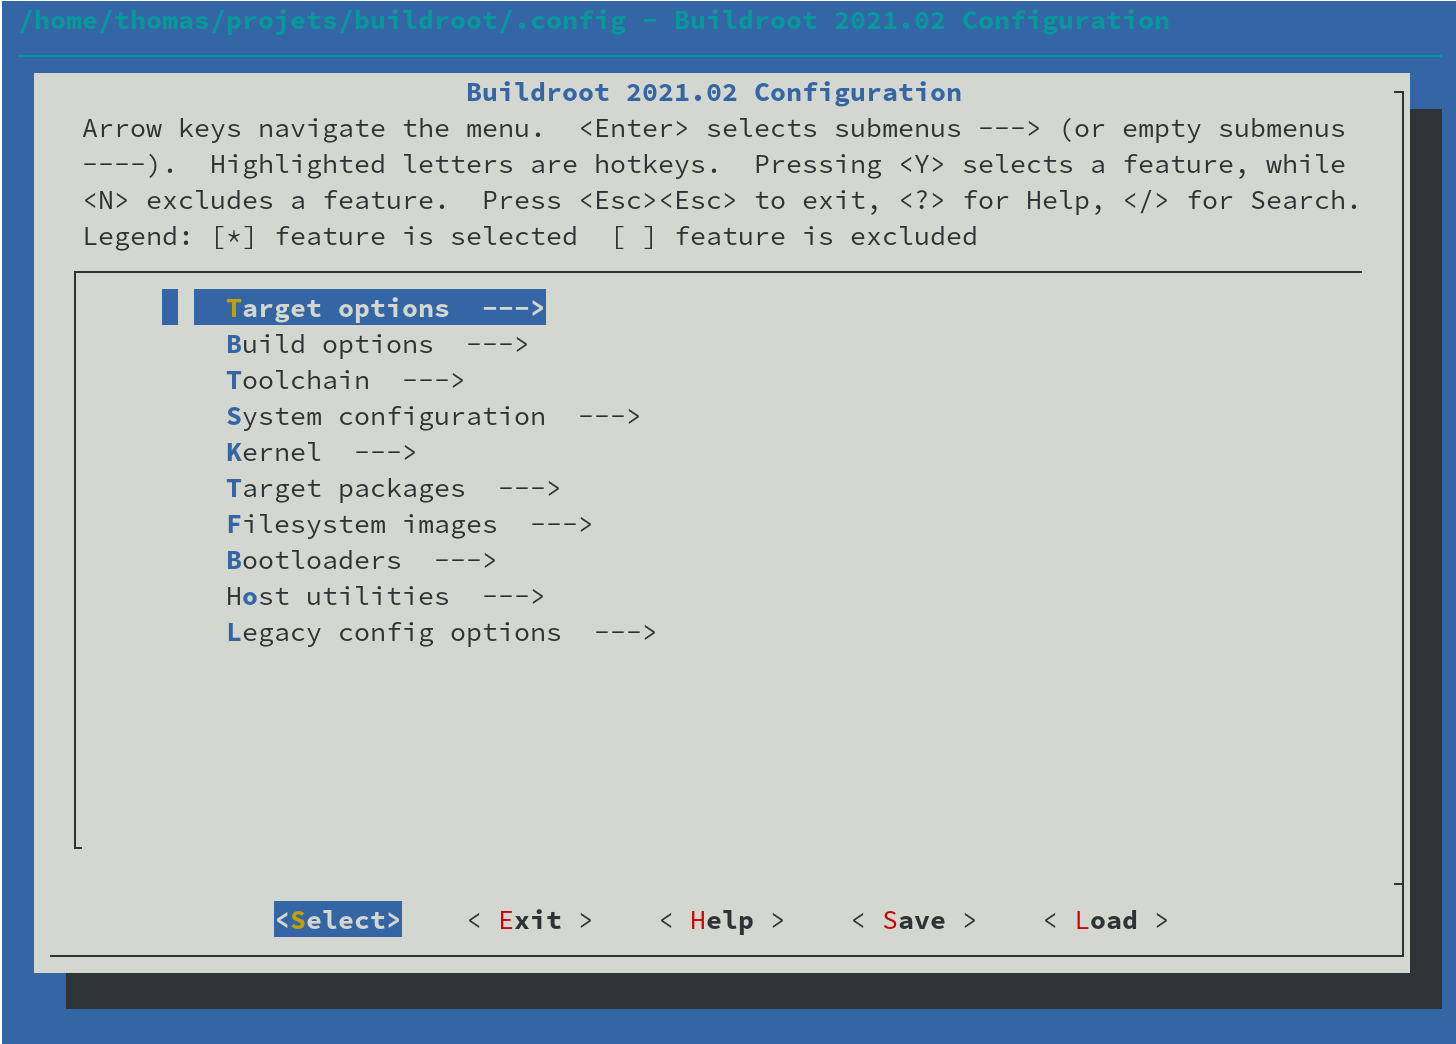
\includegraphics[height=0.8\textheight]{slides/buildroot-introduction/menuconfig.png}
  \end{center}
\end{frame}

\begin{frame}[fragile]{Running the build}
  \begin{itemize}
  \item As simple as:
    \begin{block}{}
\begin{verbatim}
$ make
\end{verbatim}
    \end{block}
  \item Often useful to keep a log of the build output, for analysis
    or investigation:
    \begin{block}{}
\begin{verbatim}
$ make 2>&1 | tee build.log
\end{verbatim}
    \end{block}
  \end{itemize}
\end{frame}

\begin{frame}{Build results}
  \begin{itemize}
  \item The build results are located in \code{output/images}
  \item Depending on the configuration, this directory will contain:
    \begin{itemize}
    \item One or several root filesystem images, in various formats
    \item One kernel image, possibly one or several Device Tree blobs
    \item One or several bootloader images
    \end{itemize}
  \item There is no standard way to install the images on any given
    device
    \begin{itemize}
    \item Those steps are very device specific
    \item Buildroot provides some tools to generate SD card / USB key
      images ({\em genimage}) or directly to flash or boot specific
      platforms: SAM-BA for Microchip, imx-usb-loader for i.MX6, OpenOCD,
      etc.
    \end{itemize}
  \end{itemize}
\end{frame}

\setuplabframe
{Basic Buildroot usage}
{
  \begin{itemize}
  \item Get Buildroot
  \item Configure a minimal system with Buildroot for the BeagleBone
    Black
  \item Do the build
  \item Prepare the BeagleBone Black for usage
  \item Flash and test the generated system
  \end{itemize}
}
